\documentclass[times, utf8, diplomski]{fer}
\usepackage{booktabs}
\usepackage{indentfirst}
\usepackage{listings}
\usepackage{amsfonts}
\usepackage{amssymb}
\usepackage{comment}
\usepackage{graphicx}
\usepackage{mdframed}
\usepackage{pdfpages}
\usepackage{amsmath}
\usepackage{array}
\usepackage{underscore}
\usepackage[section]{placeins}
\usepackage{relsize}


\begin{document}


\title{ Raspoznavanje aktivnosti osoba na temelju siluete }


\author{ \begin{tabular}{ l }
	Kuman Stipe \\
	Meštrović Stjepan \\
	Mujić Azzaro \\
	Mužar Irena \\
	Novković Igor \\
	Skukan Luka \\
	Venanzoni Andrea \\
\end{tabular}  }

\maketitle

% Dodavanje zahvale ili prazne stranice. Ako ne želite dodati zahvalu, naredbu ostavite radi prazne stranice.
\zahvala{}

\tableofcontents


\chapter{Projektni zadatak}

(do 10 stranica)

\section{Opis projektnog zadatka}

Opis problema koji zadatak obuhvaća. Što su ulazni podaci, a što zahtjevani izlaz? Koncepti/algoritmi koji se obavezno moraju upotrijebiti?

\section{Pregled i opis srodnih rješenja}

U nastavku slijedi opis radova srodnih tema koji će se koristiti kao materijal za učenje.


\subsubsection{ • Andrea Bottino, Aldo Laurentini
A silhouette based technique for the reconstruction of human movement }


Invazivni senzorni sustavi obično se temelje na magnetskom i optičkom praćenju pokreta i
podrazumijevaju veće ili manje objekte pričvršćene na tijelu izvođača i pritom ga mogu
ometati. Za neke primjene, kao što je npr. analiza sportske izvedbe, to može imati velik
negativni utjecaj. U ovom se radu opisuje neinvanzivna tehnika kojom se može rekonstruirati
prirodni pokret i kojom se nastoji riješiti navedeni problem.

Tehnikom presjeka volumena obavlja se 3D rekonstrukcija pokreta iz slika snimljenih
običnom kamerom sa različitih gledišta. Podatci o pokretu prikupljaju se projiciranjem modela
na rekonstruirani volumen.

Rekonstruiranje 3D oblika iz 2D silueta je popularan pristup u računalnom vidu. Model se
sastoji od dvije komponente: prikaza kostura i prikaza tijela koje ga okružuje. Kostur ima 15
segmenata koji su povezani zglobovima u obliku sfere. Tijelo oko kostura je prikazano sa približno
600 trokuta.

Siluete se izlučuju oduzimanjem pozadine. Presjek volumena algoritam je primjenjiv za
različite rezolucije i daje granice rekonstruiranog volumena.
Određivanje posture tijela temelji se na pretraživanju 32-dimenzionalnog prostora parametara,
i podrazumijeva pronalaženje poze modela koji najbolje aproksimira stvarni pokret.
Sustav je testiran u virtualnom okruženju i na stvarnom slijedu slika.

\subsubsection{ 
Meghna Singh, Anup Basu, Mrinal Kr. Mandal
Human activity recognition based on silhouette directionality
 }
 
I ovaj rad, također, daje opis neinvanzivne tehnike kojom se rekonstruira pokret. Koristi
adaptivnu tehnika odvajanja pozadine za izlučivanje informacija i generiranje silueta iz
snimke. Iz kontura siluete se, tada, određuju usmjereni vektori i, za grupiranje i
raspoznavanje, koristi se distribucija podataka vektora smjera. Iskorištavaju se dinamičke
karakteristike ljudskog pokreta da bi se zagladile odluke i smanjile pogreške u prepoznavanju
pokreta.

Za izdvajanje siluete koristi se statistički model pozadine, računanje očekivanja i varijance
intenziteta svakog slikovnog elementa na slici na kojoj se nalazi samo pozadina. Ta je metoda
otpornija na šum, sjenu i promjenu svjetla nego oduzimanje pozadine.

Silueta je obično pod utjecajem šuma i može se sastojati od nepovezanih komponenata. Da bi
se dobila „čista“ silueta, koriste se morfologičke operacije i analiza povezanih komponenti.
Kontura siluete prikazana je lančanim kodom iz kojeg se onda određuju vektori smjera.
Dobiveni vektori se normaliziraju. \\


Pretpostavka je da vrijedi: 


% ne isplati se enumerate
%\begin{enumerate}
%  \setcounter{enumi}{1}
%  \item
%  Normalizirani vektori smjera, za različite izvođače za iste aktivnosti na jednakoj
%udaljenosti od kamere, imaju malu varijancu.
%  \item
%   Normalizirani vektori smjera, za različite izvođače za iste aktivnosti na različitim
% od kamere i s promjenjivom pozadinom, imaju malu varijancu.
%	\item
%	Varijanca normaliziranih vektora smjera za različite aktivnosti je velika.
%\end{enumerate}


1. Normalizirani vektori smjera, za različite izvođače za iste aktivnosti na jednakoj
udaljenosti od kamere, imaju malu varijancu.

2. Normalizirani vektori smjera, za različite izvođače za iste aktivnosti na različitim
udaljenostima od kamere i s promjenjivom pozadinom, imaju malu varijancu.

3. Varijanca normaliziranih vektora smjera za različite aktivnosti je velika.
\newline

Vektori se grupiraju k-centroid algoritmom grupiranja (eng. k-means clustering).
Zbog mogućeg lošeg izdvajanja siluete, može doći do velikih varijanci vektora smjera
susjednih okvira i uzrokovati pogrešne odluke te se, stoga, koristi zaglađivanje.
Točnost algoritma varira između 85\% i 99\% za osam aktivnosti, kada se ne koristi
zaglađivanje. Kada se koriti zaglađivanje, točnost raste na 100\%.
Ovaj algoritam dobro radi i za periodični i za neperiodični pokret, ne koristi uspoređivanje
predložaka i ne zahtjeva praćenje povijesti za raspoznavanje. Algoritam se koristi za
određivanje pet osnovnih aktivnosti: uspravno stajanje, sjedenje, čučanje, ležanje i
pokazivanje.


\subsubsection{ Liang Wang, Weiming Hu, Tieniu Tan
Recent developments in human motion analysis
 }

U ovom se radu daje opsežan opis radova sa područja ljudskog pokreta od 1989. do danas.
Fokusira se na općeniti pregled aktivnosti koje uključuje analiza ljudskog pokreta:
detektiranje, praćenje čovjeka te razumijevanje ljudskog ponašanja.

Detekcija čovjeka podrazumijeva odvajanje segmenta slike koji se odnosi na čovjeka od
ostatka slike. Oduzimanje pozadine jedna je od popularnijih metoda segmentacije pokreta,
posebice u slučajevima relativno statične pozadine. S druge strane, statističke metode koriste
slikovni element ili grupe slikovnih elemenata za konstruiranje naprednijih pozadinskih
modela, a statistika pozadine se može dinamički ažurirati.

Cilj klasifikacije objekta u pokretu je odvojiti područje koje odgovara čovjeku od svih ostalih
objekata navedenim metodama segmentacije. Dvije su glavne kategorije: klasifikacija na
temelju oblika i klasifikacija na temelju pokreta.

Praćenje pokreta služi za pripremu procjene poze i raspoznavanje akcije. Može se podijeliti na
četiri kategorije: praćenje na temelju modela (model kostura, 2D konture, volumni modeli),
praćenje na temelju područja, praćenje na temelju aktivne konture te praćenje na temelju
značajki.

Razumijevanje ljudskog pokreta uključuje raspoznavanje akcija te njihov opis. Opće tehnike
koje se koriste za usporedbu vremenski zavisnih podataka su: dinamično savijanje vremena
(eng. Dynamic time-warping), skriveni markovljevi modeli i neuronske mreže. Metode za
raspoznavanje akcija su: uspoređivanje predložaka, pristup prostoru stanja i semantički opis.

\section{Konceptualno rješenje zadatka}

\subsection{Baza}

Baza koju ćemo koristiti će biti Weizman baza. Baza se sastoji od 90 snimaka podijeljenih u
10 aktivnosti, znači sadrži 9 snimaka za svaku aktivnost. Aktivnosti sadržane u bazi koje se
mogu prepoznavati su: \\
• hodanje, \\
• trčanje, \\
• skakanje, \\
• hodanje u stranu, \\
• savijanje, \\
• mahanje jednom rukom, \\
• mahanje s obje ruke, \\
• skakanje na mjestu, \\
• skakanje s ispruženim rukama, \\
• preskakivanje. \\

Snimke su snimane statičnom kamerom rezolucije 180 x 144 piksela. Na snimkama je
prisutan šum u obliku hodanja s psom ili nošenja torbe. Snimke sadrže homogenu pozadinu
radi lakšeg izdvajanja pozadine od siluete.
\newline
\begin{figure}[ht!]
\centering
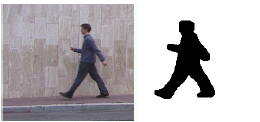
\includegraphics[width=60mm]{walk.png}
\caption{ Primjer hodanja i pripadne siluete \label{overflow}}
\end{figure}


Primjer hodanja i pripadne siluete
U aplikaciji nećemo koristiti sve aktivnosti za prepoznavanje, već ćemo se, radi
jednostavnosti, ograničiti na dvije ili tri aktivnosti. Na slikama 1.1 i 1.2 mogu se vidjeti
primjeri snimaka hodanja i trčanja i pripadnih silueta.
\newline
\begin{figure}[ht!]
\centering
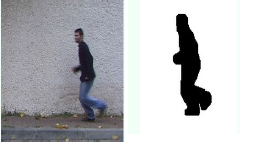
\includegraphics[width=60mm]{run.png}
\caption{ Primjer trčanja i pripadne siluete \label{overflow}}
\end{figure}


\subsection{Arhitektura sustava}

Sustav možemo podjeliti na sljedećih 5 modula: \\
• izdvajanje siluete, \\
• reprezentacija siluete, \\
• izdvajanje vektora značajki i normalizacija, \\
• klasifikacija, \\
• vremensko zaglađivanje \\
Slika 1.3 prikazuje blok shemu sustava.
\newline
\begin{figure}[ht!]
\centering
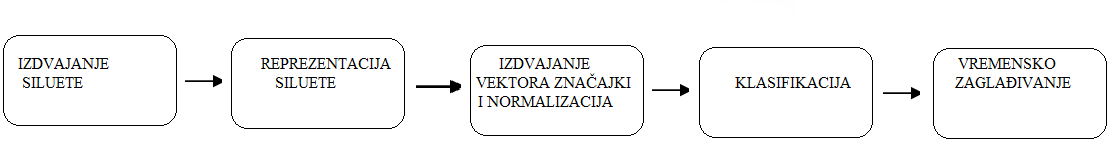
\includegraphics[width=170mm]{arhitektura.png}
\caption{ Blok shema sustava \label{overflow}}
\end{figure}

Ulaz u sustav je snimka na kojoj osoba obavlja određenu aktivnost. Na svakoj slici snimke se
izdvaja silueta od pozadine. Prije izdvajanja siluete slika se iz RGB sustava prebacuje u sustav
intenziteta sive boje postupkom određivanja prosjeka R, G i B komponente. Silueta se izdvaja
od pozadine statistickim modelom pozadine, gdje se računa očekivanje i varijanca svakog
piksela pozadine početnih N slika, na kojima osoba nije prisutna. Ova metoda je robusnija od
jednostavnijih metoda, poput oduzimanja pozadine. Za svaki piksel se računa prag kao
maksimalna razlika očekivanja i intenziteta sive boje kod početnih N slika. Pripada li piksel
silueti se određuje na sljedeći način: 
\newline
• ako je razlika intenziteta piksela i očekivanja intenziteta piksela manja od praga, piksel
pripada pozadini, \\
• inače piksel pripada silueti \\
\newline
\begin{figure}[ht!]
\centering
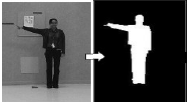
\includegraphics[width=60mm]{pozadina1.png}
\caption{ Izdvajanje siluete od pozadine \label{overflow}}
\end{figure}



Zatim se izlučuje kontura siluete primjenom Gauss-ovog filtra. Izlaz prvog modula je slika
koja sadrži konturu siluete.
\newline
\begin{figure}[ht!]
\centering
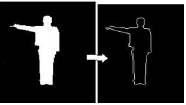
\includegraphics[width=60mm]{pozadina2.png}
\caption{ Izlučivanje konture siluete \label{overflow}}
\end{figure}



Drugi modul radi reprezentaciju konture siluete pomoću lančanog koda. Lančani kod govori
u koju stranu se moramo pomaknuti da od jednog piksela konture dođemo do sljedećeg
piksela konture. Na slici 1.6 prikazan je lančani kod sa sljedećim oznakama: \\
• kod 0 ima piksel koji je iznad trenutnog piksela, \\
• kod 1 ima piksel koji je gore-desno od trenutnog piksela, \\
• kod 2 ima piksel koji je desno od trenutnog piksela, \\
• kod 3 ima piksel koji je dolje-desno od trenutnog piksela, \\
• kod 4 ima piksel koji je ispod trenutnog piskela, \\
• kod 5 ima piksel koji je dolje-lijevo od trenutnog piksela, \\
• kod 6 ima piksel koji je lijevo od trenutnog piksela, \\
• kod 7 ima piksel koji je gore-lijevo od trenutnog piksela \\
\newline
\begin{figure}[ht!]
\centering
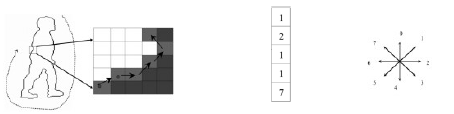
\includegraphics[width=160mm]{lancanikod.png}
\caption{ Prikaz lančanog koda \label{overflow}}
\end{figure}


Obilaženjem cijele konture siluete dobiva se vektor lančanog koda koji je izlaz ovog modula.
Sljedeći modul grupira vektor lančanog koda u 8-dimenzionalni usmjereni vektor. Grupacija
se radi na temelju frekvencije pojavljivanja koda. Radi postizanja robusnosti usmjereni
vektori se normaliziraju. Za svaki par slika, određuje se veličina kuta između normaliziranih
vektora tih slika, te se ti kutevi šalju kao ulaz u sljedeći modul.

Za svrhu klasificiranja koristimo k-centroidni algoritam grupiranja (eng. k-means clustering
algorithm). Pošto algoritam grupiranja spada pod model nenadziranog učenja, prvo ćemo
odrediti centroide snimaka na kojima znamo koja se aktivnost odvija. Zatim će se na
nepoznatim primjerima klasifikacija vršiti uzimanjem minimalne udaljenosti centroida.

Ako se između dvije slike aktivnost naglo promijeni, moguće je da je riječ o pogrešci.
Pogreška se može dogoditi ako se loše izdvojila silueta od pozadine. Tada se uspoređuje slika
na kojoj se pogreška dogodila sa slikama prije i nakon nje.

 Izračunavaju se nove vrijednosti piksela slike kao prosjek vrijednosti piksela slika prije i nakon nje. Na takvoj slici sa izračunatim novim vrijednostima piksela se vrši ponovna klasifikacija.



\chapter{Postupak rješavanja zadatka}

(do 10 stranica)

Navesti numerirani slijed koraka rješavanja. Npr.: 1. Dobivanje binarne slike iz slike u boji, 2. Segmentacija objekata na slici, 3. Nalaženje rubova u slici ...

\section{Izdvajanje pozadine}

Prvi korak postupka prepoznavanje aktivnosti osobe je izdvajanje siluete osobe od pozadine. Ulaz ovog modula je snimka rezolucije 180 x 144, a izlaz modula je snimka na kojoj je silueta označena bijelom bojom a pozadina crnom bojojm

\subsection{Transformacija slike u boji u sliku intenziteta}

Prvi korak izdvajanja pozadine je pretvorba slike u boji u sliku intenziteta sive boje. Na taj način se postize manja razlika vrijednosti piksela te se odvajanje siluete od pozadine može provesti uspješnije. Transformacija se provodi upotrebom CCIR 601 standarda. Standard CCIR 601 prilikom transformacije sustava uzima u obzir da ljudsko oko ne vidi svaku boju jednako, neke boje vidi intenzivnije a neke slabije. Ljudsko oko zelenu boju percipira najintezivnije, potom crvenu pa plavu. U skladu s tim transformacija se vrši otežanom sumom vrijednosti intenziteta crvene, zelene i plave boje na sljedeći način:

$$ Y = 0.299 \cdot R + 0.587 \cdot G + 0.114 \cdot B. $$

\subsection{Statistički model izdvajanja pozadine}

Nakon dobivanja slike u intenzitetu sive boje, nad slikom se provodi postupak izdvajanje pozadine statističkim modelom. Statistički model se definira izračunom varijance i očekivanja intenziteta svakog piksela. Pretpostavka je da u početnih N slika snimke će se prikazivati samo pozadina, te se varijanca i očekivanje računaju na tih N početnih slika na sljedeći način:

	$$u(x,y) = \frac{1}{N} \cdot  \sum (p(x,y;i)),$$

\vspace{0.4cm}

gdje je u(x,y) očekivanje intenzite piksela na pozixiji x,y, p(x,y;i) je vrijednost intenziteta piksela na pozicij x,y na slici i. Time se dobiva robusnost i točnije prepoznavanje u odnosu na jednostavnije modele oduzimanja pozadine. Nakon određivanja varijance i očekivanja intenziteta svakog piksela određuje se prag intenziteta kojeg mora preći piksel na novoj slici da bi se smatrao pikselom siluete. Prag se određuje kao maksimalna razlika očekivanja intenziteta pojedinog piksela i vrijednosti piksela na početnim slikama na temelju kojih se računala varijanca i očekivanje.

$$T(x,y) = \max{ \big|u(x,y) - p(x,y;i)\big|}, 1 \leq i \leq N,$$

gdje je T(x,y) prag intenziteta piksela x,y.

Potom se na slikama na kojima je objekt prisutan pripadnost piksela klasificira na sljedeći način:
\newline
  Ako: 
  $$ \big|p(x,y;k - u(x,y)\big| < T(x,y),$$
      zaključujemo da piksel pripada pozadini,
  a inače piksel pripada silueti
      
Prednost ovog načina izdvajanja pozadine je već spomenuta robusnost zbog mogućnosti izgradnje razdiobe za svaki piksel slike. No u slučaju da je objekt prisutan od prve slike, moguće su pogreške u izdvajanju pozadine u prvih par slika jer nije određrena razdioba intenziteta.


\section{Reprezentacija siluete}

\section{Izlučivanje vektora značajki}

\section{Klasifikacija}


\section{Vremensko zaglađivanje}

\chapter{Ispitivanje rješenja}

(do 10 stranica)

\section{Ispitna baza}

Opisati ispitnu bazu, tipove i broj različitih uzoraka u bazi te na koji su način uzorci iz baze korišteni prilikom učenja i ispitivanja rješenja projektnog zadatka. 

\section{Rezultati učenja i ispitivanja}

Prikazati statističke podatke o uspješnosti rješenja prilikom učenja/ispitivanja te opisati eksperimente na temelju kojih su podaci dobiveni.

\section{Analiza rezultata}

Analizirati uzroke rezultata ispitivanja, povezati sa uzorcima u bazi i algoritmima korištenim u rješenju. Raspraviti moguća poboljšanja.

\chapter{Opis programske implementacije rješenja}

(do 5 stranice)

Opisati sučelje programske implementacije i način korištenja implementacije.


\chapter{Zaključak}

(do 2 stranice)

Ocijeniti uspješnost implementacije, navesti budući rad u smislu potrebnih poboljšanja. 


\chapter{Literatura}

1. Ime i prezime autora: Naziv časopisa vol. br. godina izdanja, pp od-do (npr. pp 486-492)/knjige/članka/web resursa (s linkom i datumom pristupa web resursu)
...
.
.
DVD/CD  
.
kompletan tekst projekta
izvorni kod projekta
exe verzija
readme file – upute za korištenje i pokretanje programa
.
baze slika (sve koje su korištene)
E-oblik članaka koji su korišteni za izradu projekta
primjeri obrade
..





%%\bibliography{literatura}
%%\bibliographystyle{fer}

\begin{sazetak}
Sažetak na hrvatskom jeziku.

\kljucnerijeci{Ključne riječi, odvojene zarezima.}
\end{sazetak}

% TODO: Navedite naslov na engleskom jeziku.
\engtitle{Title}
\begin{abstract}
Abstract.

\keywords{Keywords.}
\end{abstract}

\end{document}
